\documentclass[10pt]{article}
\usepackage[T1]{fontenc}

% Document Details
\newcommand{\CLASS}{AMATH 586}
\newcommand{\assigmentnum}{Assignment 5}

\usepackage[margin = 1.15in, top = 1.25in, bottom = 1.in]{geometry}

\usepackage{titling}
\setlength{\droptitle}{-6em}   % This is your set screw
\date{}
\renewcommand{\maketitle}{
	\clearpage
	\begingroup  
	\centering
	\LARGE \sffamily\textbf{\CLASS} \Large \assigmentnum\\[.8em]
	\large Tyler Chen\\[1em]
	\endgroup
	\thispagestyle{empty}
}
 % Title Styling
\usepackage{tocloft}
\renewcommand{\cfttoctitlefont}{\Large\sffamily\bfseries}
\renewcommand{\cftsecfont}{\normalfont\sffamily\bfseries}
\renewcommand{\cftsubsecfont}{\normalfont\sffamily}
\renewcommand{\cftsubsubsecfont}{\normalfont\sffamily}

\makeatletter
\let\oldl@section\l@section
\def\l@section#1#2{\oldl@section{#1}{\sffamily\bfseries#2}}

\let\oldl@subsection\l@subsection
\def\l@subsection#1#2{\oldl@subsection{#1}{\sffamily#2}}

\let\oldl@subsubsection\l@subsubsection
\def\l@subsubsection#1#2{\oldl@subsubsection{#1}{\sffamily#2}}
 % General Styling


\usepackage{enumitem}

% Figures
\usepackage{subcaption}

% TikZ and Graphics
\usepackage{tikz, pgfplots}
\pgfplotsset{compat=1.12}
\usetikzlibrary{patterns,arrows}
\usepgfplotslibrary{fillbetween}

\usepackage{pdfpages}
\usepackage{adjustbox}

\usepackage{lscape}
\usepackage{titling}
\usepackage[]{hyperref}


% Header Styling
\usepackage{fancyhdr}
\pagestyle{fancy}
\lhead{\sffamily \CLASS}
\rhead{\sffamily Chen \textbf{\thepage}}
\cfoot{}

% Paragraph Styling
\setlength{\columnsep}{1cm}
\setlength{\parindent}{0pt}
\setlength{\parskip}{5pt}
\renewcommand{\baselinestretch}{1}

% TOC Styling
\usepackage{tocloft}
\iffalse
\renewcommand{\cftsecleader}{\cftdotfill{\cftdotsep}}

\renewcommand\cftchapafterpnum{\vskip6pt}
\renewcommand\cftsecafterpnum{\vskip10pt}
\renewcommand\cftsubsecafterpnum{\vskip6pt}

% Adjust sectional unit title fonts in ToC
\renewcommand{\cftchapfont}{\sffamily}
\renewcommand{\cftsecfont}{\bfseries\sffamily}
\renewcommand{\cftsecnumwidth}{2em}
\renewcommand{\cftsubsecfont}{\sffamily}
\renewcommand{\cfttoctitlefont}{\hfill\bfseries\sffamily\MakeUppercase}
\renewcommand{\cftaftertoctitle}{\hfill}

\renewcommand{\cftchappagefont}{\sffamily}
\renewcommand{\cftsecpagefont}{\bfseries\sffamily}
\renewcommand{\cftsubsecpagefont}{\sffamily}
\fi
 % General Styling
% Code Display Setup
\usepackage{listings,lstautogobble}
\usepackage{lipsum}
\usepackage{courier}
\usepackage{catchfilebetweentags}

\lstset{
	basicstyle=\small\ttfamily,
	breaklines=true, 
	frame = single,
	rangeprefix=,
	rangesuffix=,
	includerangemarker=false,
	autogobble = true
}


\usepackage{algorithmicx}
\usepackage{algpseudocode}

\newcommand{\To}{\textbf{to}~}
\newcommand{\DownTo}{\textbf{downto}~}
\renewcommand{\algorithmicdo}{\hspace{-.2em}\textbf{:}}
 % Code Display Setup
% AMS MATH Styling
\usepackage{amsmath, amssymb}
\newcommand{\qed}{\hfill\(\square\)}

%\newtheorem*{lemma}{Lemma} 
%\newtheorem*{theorem}{Theorem}
%\newtheorem*{definition}{Definition}
%\newtheorem*{prop}{Proposition}
%\renewenvironment{proof}{{\bfseries Proof.}}{}


% mathcal
\newcommand{\cA}{\ensuremath{\mathcal{A}}}
\newcommand{\cB}{\ensuremath{\mathcal{B}}}
\newcommand{\cC}{\ensuremath{\mathcal{C}}}
\newcommand{\cD}{\ensuremath{\mathcal{D}}}
\newcommand{\cE}{\ensuremath{\mathcal{E}}}
\newcommand{\cF}{\ensuremath{\mathcal{F}}}
\newcommand{\cG}{\ensuremath{\mathcal{G}}}
\newcommand{\cH}{\ensuremath{\mathcal{H}}}
\newcommand{\cI}{\ensuremath{\mathcal{I}}}
\newcommand{\cJ}{\ensuremath{\mathcal{J}}}
\newcommand{\cK}{\ensuremath{\mathcal{K}}}
\newcommand{\cL}{\ensuremath{\mathcal{L}}}
\newcommand{\cM}{\ensuremath{\mathcal{M}}}
\newcommand{\cN}{\ensuremath{\mathcal{N}}}
\newcommand{\cO}{\ensuremath{\mathcal{O}}}
\newcommand{\cP}{\ensuremath{\mathcal{P}}}
\newcommand{\cQ}{\ensuremath{\mathcal{Q}}}
\newcommand{\cR}{\ensuremath{\mathcal{R}}}
\newcommand{\cS}{\ensuremath{\mathcal{S}}}
\newcommand{\cT}{\ensuremath{\mathcal{T}}}
\newcommand{\cU}{\ensuremath{\mathcal{U}}}
\newcommand{\cV}{\ensuremath{\mathcal{V}}}
\newcommand{\cW}{\ensuremath{\mathcal{W}}}
\newcommand{\cX}{\ensuremath{\mathcal{X}}}
\newcommand{\cY}{\ensuremath{\mathcal{Y}}}
\newcommand{\cZ}{\ensuremath{\mathcal{Z}}}

% mathbb
\usepackage{bbm}
\newcommand{\bOne}{\ensuremath{\mathbbm{1}}}

\newcommand{\bA}{\ensuremath{\mathbb{A}}}
\newcommand{\bB}{\ensuremath{\mathbb{B}}}
\newcommand{\bC}{\ensuremath{\mathbb{C}}}
\newcommand{\bD}{\ensuremath{\mathbb{D}}}
\newcommand{\bE}{\ensuremath{\mathbb{E}}}
\newcommand{\bF}{\ensuremath{\mathbb{F}}}
\newcommand{\bG}{\ensuremath{\mathbb{G}}}
\newcommand{\bH}{\ensuremath{\mathbb{H}}}
\newcommand{\bI}{\ensuremath{\mathbb{I}}}
\newcommand{\bJ}{\ensuremath{\mathbb{J}}}
\newcommand{\bK}{\ensuremath{\mathbb{K}}}
\newcommand{\bL}{\ensuremath{\mathbb{L}}}
\newcommand{\bM}{\ensuremath{\mathbb{M}}}
\newcommand{\bN}{\ensuremath{\mathbb{N}}}
\newcommand{\bO}{\ensuremath{\mathbb{O}}}
\newcommand{\bP}{\ensuremath{\mathbb{P}}}
\newcommand{\bQ}{\ensuremath{\mathbb{Q}}}
\newcommand{\bR}{\ensuremath{\mathbb{R}}}
\newcommand{\bS}{\ensuremath{\mathbb{S}}}
\newcommand{\bT}{\ensuremath{\mathbb{T}}}
\newcommand{\bU}{\ensuremath{\mathbb{U}}}
\newcommand{\bV}{\ensuremath{\mathbb{V}}}
\newcommand{\bW}{\ensuremath{\mathbb{W}}}
\newcommand{\bX}{\ensuremath{\mathbb{X}}}
\newcommand{\bY}{\ensuremath{\mathbb{Y}}}
\newcommand{\bZ}{\ensuremath{\mathbb{Z}}}

% alternative mathbb
\newcommand{\NN}{\ensuremath{\mathbb{N}}}
\newcommand{\RR}{\ensuremath{\mathbb{R}}}
\newcommand{\CC}{\ensuremath{\mathbb{C}}}
\newcommand{\ZZ}{\ensuremath{\mathbb{Z}}}
\newcommand{\EE}{\ensuremath{\mathbb{E}}}
\newcommand{\PP}{\ensuremath{\mathbb{P}}}
\newcommand{\VV}{\ensuremath{\mathbb{V}}}
\newcommand{\cov}{\ensuremath{\text{Co}\VV}}
% Math Commands

\newcommand{\st}{~\big|~}
\newcommand{\stt}{\text{ st. }}
\newcommand{\ift}{\text{ if }}
\newcommand{\thent}{\text{ then }}
\newcommand{\owt}{\text{ otherwise }}

\newcommand{\norm}[1]{\left\lVert#1\right\rVert}
\newcommand{\snorm}[1]{\lVert#1\rVert}
\newcommand{\ip}[1]{\ensuremath{\left\langle #1 \right\rangle}}
\newcommand{\pp}[3][]{\frac{\partial^{#1}#2}{\partial #3^{#1}}}
\newcommand{\dd}[3][]{\frac{\d^{#1}#2}{\d #3^{#1}}}
\renewcommand{\d}{\ensuremath{\mathrm{d}}}

\newcommand{\indep}{\rotatebox[origin=c]{90}{$\models$}}




 % Math shortcuts
% Problem
\usepackage{floatrow}

\newenvironment{problem}[1][]
{\pagebreak
\noindent\rule{\textwidth}{1pt}\vspace{0.25em}
{\sffamily \textbf{#1}}
\par
}
{\par\vspace{-0.5em}\noindent\rule{\textwidth}{1pt}}

\newenvironment{solution}[1][]
{{\sffamily \textbf{#1}}
\par
}
{}

 % Problem Environment

\newcommand{\note}[1]{\textcolor{red}{\textbf{Note:} #1}}

\hypersetup{
   colorlinks=true,       % false: boxed links; true: colored links
   linkcolor=violet,          % color of internal links (change box color with linkbordercolor)
   citecolor=green,        % color of links to bibliography
   filecolor=magenta,      % color of file links
   urlcolor=cyan           % color of external links
}


\begin{document}
\maketitle



\begin{problem}[Problem 1]
Let \(A_{\epsilon}\) be the \(m+1\) by \(m+1\) matrix
\[
A_{\epsilon} = - \frac{a}{2h} \left[ \begin{array}{cccc}
0 & 1 &        & -1 \\
-1 & \ddots & \ddots & \\
   & \ddots & \ddots & 1 \\
1  &        & -1     & 0 \end{array} \right] + \frac{\epsilon}{h^2} \left[ \begin{array}{cccc}
-2 & 1 & & 1 \\
1 & \ddots & \ddots & \\
  & \ddots & \ddots & 1 \\
1 &        & 1      & -2 \end{array} \right] ,
\]
as in (10.15).  Show that the eigenvalues of \(A_{\epsilon}\) are
\[
\mu_p = - \frac{ia}{h} \sin ( 2 \pi p h ) - \frac{2 \epsilon}{h^2} ( 1 - \cos ( 2 \pi p h )) ,
~~p=1, \ldots ,m+1 ,
\]
where \(h = \frac{1}{m+1}\), and that the corresponding eigenvectors are
\[
u_j^p = e^{2 \pi i p j h} ,~~j=1, \ldots , m+1 .
\]
\end{problem}

\begin{solution}[Solution]

Write,
\begin{align*}
    A_1 = \left[ \begin{array}{cccc}
    0 & 1 &  & -1 \\
    -1 & \ddots & \ddots & \\
       & \ddots & \ddots & 1 \\
    1  &  & -1  & 0 \end{array} \right]
    ,&&
    A_2 = \left[ \begin{array}{cccc}
    0 & 1 &  & 1 \\
    1 & \ddots & \ddots & \\
       & \ddots & \ddots & 1 \\
    1  &  & 1  & 0 \end{array} \right]
\end{align*}

Recall that for any integer \( k \),
\begin{align*}
    \exp\left(\dfrac{2\pi i z}{m+1}\right) = \exp\left(\dfrac{2\pi i (z+k(m+1))}{m+1}\right)
\end{align*}

Let \( [z] \) denote all integers equivalent to \( z \) modulo \( m+1 \). When using \( [z] \) in an expression, we mean pick any integer from this equivalence class.
Then,
\begin{align*}
    (A_1 u^p)_{j} %= \sum_{k=1}^{m+1} (A_1)_{jk} u_k^p
    &= \left( \exp \left( \dfrac{2\pi i p [j+1]}{m+1} \right) - \exp \left( \dfrac{2\pi i p [j-1]}{m+1} \right) \right) \\
    &= \left( \exp \left( \dfrac{2\pi i p}{m+1} \right)- \exp \left(-\dfrac{2\pi i p}{m+1} \right)  \right) \exp \left( \dfrac{2\pi i p j}{m+1} \right) \\
    &= 2i\sin \left( \dfrac{2\pi p}{m+1} \right) \exp \left( \dfrac{2\pi i p j}{m+1} \right)
\end{align*}

Similarly,
\begin{align*}
    (A_2 u^p)_{j} %= \sum_{k=1}^{m+1} (A_1)_{jk} u_k^p
    &= \left( \exp \left( \dfrac{2\pi i p [j+1]}{m+1} \right) + \exp \left( \dfrac{2\pi i p [j-1]}{m+1} \right) \right) \\
    &= \left( \exp \left( \dfrac{2\pi i p}{m+1}\right) + \exp \left(-\dfrac{2\pi i p}{m+1} \right) \right) \exp \left( \dfrac{2\pi i p j}{m+1} \right) \\
    &= 2 \cos \left( \dfrac{2\pi p}{m+1} \right) \exp \left( \dfrac{2\pi i p j}{m+1} \right)
\end{align*}

This proves that for any integer \( p \), \( u^p = \exp(2\pi i p j h) \) is an eigenvector of \( A_1 \) and \( A_2 \) with eigenvalues \( 2i\sin(2\pi p h) \) and \( 2\cos(2\pi p h) \) respectively. Clearly \( u^p \) is an eigenvector of \( -2I_{m+1} \) with eigenvalue \( -2 \).

Finally, observe,
\begin{align*}
    A_{\epsilon} = -\dfrac{a}{2h}A_1 + \dfrac{\epsilon}{h^2} \left( A_2-2 I_{m+1} \right)
\end{align*}

It follows that \( u^p \) is an eigenvector of \( A_\varepsilon \) with eigenvalue,
\begin{align*}
    -\dfrac{a}{2h} \left( 2i\sin \left( \dfrac{2\pi p j}{m+1} \right)  \right) + \dfrac{\epsilon}{h^2} \left( 2 \cos \left( \dfrac{2\pi p j}{m+1} \right)-2 \right) = -\dfrac{ia}{h}\sin(2\pi p h) - \dfrac{2\epsilon}{h^2}\left( 1-\cos(2\pi p h) \right) \tag*{\qed}
\end{align*}


\end{solution}

\begin{problem}[Problem 2]
Suppose \(a > 0\) and consider the following {\em skewed leapfrog} method for solving the advection equation \(u_t + a u_x = 0\):
\[
U_j^{n+1} = U_{j-2}^{n-1} - \left( \frac{ak}{h} - 1 \right) ( U_j^n - U_{j-2}^n ) .
\]
Note that if \(ak/h \approx 1\) then the stencil of this method roughly follows the characteristic of the advection equation (\(x-at = \mbox{constant}\)) and might be expected to be more accurate than standard leapfrog.  (Like other methods we have studied, if \(ak/h = 1\) the method is exact.)
\begin{enumerate}[label=(\alph*)]
\item What is the order of accuracy of this method?
\item For what range of Courant number \(ak/h\) does this method satisfy the CFL condition?
\item Show that the method is in fact stable for this range of Courant numbers by doing von Neumann analysis.
[Hint:  Let \(\gamma ( \xi ) = e^{i h \xi} g( \xi )\) and show that \(\gamma ( \xi )\) satisfies a quadratic equation closely related to the equation (10.34) that arises from a von Neumann analysis of the leapfrog method.]
\item Produce a plot similar to those in Figure 10.4 using this method with \(a=1\), \(h=0.05\) and \(k=0.8 h\).
\end{enumerate}
\end{problem}

\begin{solution}[Solution]

\begin{enumerate}[label=(\alph*)]
    \item We rearrange this to,
    \begin{align*}
        \dfrac{1}{2} \left( \dfrac{U_{j}^{n+1} - U_j^n}{k} + \dfrac{U_{j-2}^n-U_{j-2}^{n-1}}{k} \right) + a \left( \dfrac{U_{j}^{n} - U_{j-2}^{n} }{2h} \right) = 0
    \end{align*}

    The local truncation error is then,
    \begin{align*}
        \tau(x,t) = \dfrac{1}{2} \left( \dfrac{u(x,t+k) - u(x,t)}{k} + \dfrac{u(x-2h,t)-u(x-2h,t-k)}{k} \right)
        + a \left( \dfrac{u(x,t) - u(x-2h,t)}{2h} \right)
    \end{align*}

    We know that,
    \begin{align*}
        \dfrac{1}{k}(u(x,t+k) - u(x,t))
        &= \dfrac{1}{k} \left( k u_t(x,t) + \dfrac{1}{2}k^2 u_{tt}(x,t) + \cO(k^3) \right)
        \\&= u_t(x,t) + \dfrac{1}{2}k u_{tt}(x,t) + \cO(k^2)
    \end{align*}
    \begin{align*}
        \dfrac{1}{k}(u(x-2h,t)-u(x-2h,t-k))
        &= \dfrac{1}{k} \left( ku_t(x-2h,t) - \dfrac{1}{2}k^2 u_{tt}(x-2h,t) + \cO(k^3) \right)
        \\&= u_t(x-2h,k) - \dfrac{1}{2}k u_{tt}(x-2h,t) + \cO(k^2)
    \end{align*}
    \begin{align*}
        \dfrac{1}{2h}\left( u(x,t) - u(x-2h,t) \right)
        &= \dfrac{1}{2h}\left( 2h u_x(x,t) - \dfrac{1}{2}(2h)^2u_{xx}(x,t) + \cO(h^3) \right)
        \\&= u_x(x,t) - hu_{xx}(x,t) + \cO(h^2)
    \end{align*}

    Putting this together we have,
    \begin{align*}
        \tau(x,t) = \dfrac{1}{2} \left( u_t(x,t) + u_t(x-2h,t) + \dfrac{k}{2}\left( u_{tt}(x,t)-u_{tt}(x-2h,t) \right) + \cO(k^2)\right) + a \left( u_x(x,t) - hu_{xx}(x,t) + \cO(h^2) \right)
    \end{align*}

    Now observe,
    \begin{align*}
        u_t(x,t) + u_t(x-2h,t) = 2u_t(x,t) - 2hu_{tx}(x,t) + 2h^2u_{txx}(x,t) + \cO(h^2)
    \end{align*}
    \begin{align*}
        \dfrac{k}{2}(u_{tt}(x,t) - u_{tt}(x-2h,t)) = \dfrac{k}{2}(2hu_{ttx}(x,t) + \cO(h^2)) = 0 + \cO(hk) %khu_{txx}(x,t) + \cO(kh^2)
    \end{align*}

    Thus,
    \begin{align*}
        \tau(x,t)  &= \dfrac{1}{2} \left( 2u_t(x,t) - 2hu_{tx}(x,t) + \cO(h^2)  + \cO(kh) \right)
        + a\left( u_x(x,t) - hu_{xx}(x,t) + \cO(h^2) \right)
        \\&= u_t(x,t) + au_x(x,t) - h(u_{tx}(x,t)+au_{xx}(x,t)) + \cO(h^2) + \cO(kh) + \cO(k^2)
        \\&= \cO(h^2) + \cO(kh) + \cO(k^2)
    \end{align*}

    \item
    \begin{figure}[H]\centering
    \begin{subfigure}{.48\textwidth}\centering
    \begin{tikzpicture}
        \draw[fill=black] (1,1) node[below] {\((x_j,t_{n+1} )\)} circle (2pt);
        \draw[fill=black] (1,0) node[below] {\((x_j,t_n)\)} circle (2pt);
        \draw[fill=black] (-1,0) node[below] {\((x_{j-2},t_n)\)} circle (2pt);
        \draw[fill=black] (-1,-1) node[below] {\((x_{j-2},t_{n-1})\)} circle (2pt);
        \foreach \x in {-1,0,1}{
        \draw[gray] (\x,-2) -- (\x,2);
        \draw[gray] (-2,\x) -- (2,\x);
        }
    \end{tikzpicture}
    \caption{Dependence grid points for leapfrog method.}
    \label{leapfrog_mesh}
    \end{subfigure}\hfill
    \begin{subfigure}{.48\textwidth}\centering
    \begin{tikzpicture}[scale=0.25]
        \def \n {20}
        \def \nn {10}
        \foreach \x in {-4,...,\n}{
            \draw[gray] (\x+2,0) -- (\x+2,\nn);
        }
        \foreach \x in {0,...,\nn}{
            \draw[gray] (-2,\x) -- (\n+2,\x);
        }
        \foreach \x in {0,1,...,\nn}{
        \foreach \y in {0,...,\x}{
            \draw[fill = black] (2*\x,\y) circle (5pt);
            }
        }
        \draw[] (20,10) node[above] {\((x_{j},t_{n})\)} circle (10pt);
        \draw[] (20,0) node[below] {\((x_{j},0)\)} circle (10pt);
        \draw[] (0,0) node[below] {\((x_{j-2n},0)\)} circle (10pt);
    \end{tikzpicture}
    \end{subfigure}
    \caption{}
    \end{figure}

    The solution a a spatial point \( (x_j,t_{n+1}) \) depends on the solution at \( (x_{j-2},t_n) \), \( (x_j,t_n) \), and \( (x_{j-2},t_{n-1}) \) as shown in Figure~\ref{leapfrog_mesh}. Thus, as we refine the mesh with \( k/h \) fixed the dependence of a point \( (X,T) \) will be \( [X-(2h/k)T,X] \).

    The CFL condition requires,
    \begin{align*}
        X - \dfrac{2h}{k}T \leq X-aT \leq X
    \end{align*}

    This is satisfied if,
    \begin{align*}
        0 \leq \dfrac{ak}{h} \leq  2
    \end{align*}

    \item Set \( U_j^n  = g(\xi)^ne^{i\xi jh} \). Then,
    \begin{align*}
        g(\xi)^{n+1}e^{i\xi j h} = g(\xi)^{n-1} e^{i\xi (j-2) h} - \left( \dfrac{ak}{h} -1 \right) \left( g(\xi)^n e^{i\xi jh} - g(\xi)^n e^{i\xi (j-2) h} \right)
    \end{align*}

    Dividing by \( g(\xi)^{n-1}e^{i\xi (j-2) h} \) yields,
    \begin{align*}
        g(\xi)^2e^{2i\xi h} = 1 - \left( \dfrac{ak}{h} -1 \right)  \left( e^{i\xi h}-e^{-i\xi h} \right) g(\xi)e^{i\xi h}
    \end{align*}

    Setting \( \gamma(\xi) = g(\xi)e^{i\xi h} \) we have,
    \begin{align*}
        \gamma(\xi)^2 = 1 - \left( \dfrac{ak}{h} -1 \right) 2i \sin(\xi h) \gamma(\xi)
    \end{align*}

    This is of the form of 10.34 so \( |\gamma(\xi)| = |g(\xi)| \leq 1 \) provided,
    \begin{align*}
        \left| \dfrac{ak}{h} -1  \right|
        \leq 1
    \end{align*}

    If \( 0\leq ak/h \leq 2 \) then clearly the above is satisfied.


    \item
    We start with initial condition \( u(x,0) = \exp\left(-20(x-2)^2\right) + \exp\left(-(x-5)^2\right) \) on \( x\in[0,25] \).
    We assume zero boundary conditions throughout this problem (this is a reasonable assumption since the points nearest to the left and right spatial boundaries have values of {\tt 1.38...e-11} and {\tt 1.91...e-174} respectively.
    We find \( U^1 \) using forward Euler, then apply the specified skewed leapfrog until time \( t=17 \).

    Note that we use {\tt convolve1d} rather than difference matrices for convenience.
    \lstinputlisting[linerange=\#<start>-\#<end>]{hw5_2.py}

    The computed solution and actual solution are shown in Figure~\ref{wave}.

    \begin{figure}[H]\centering
        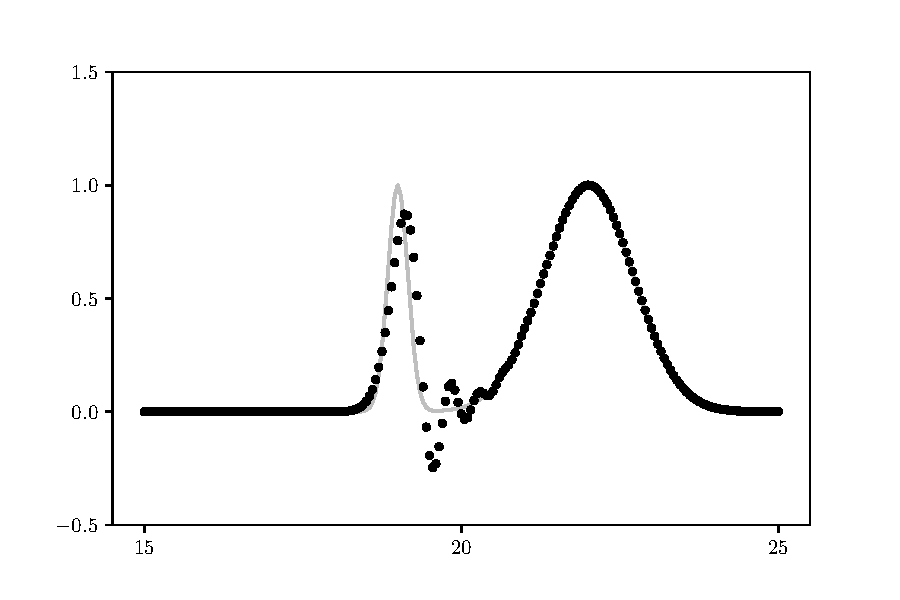
\includegraphics[width=.8\textwidth]{wave.pdf}
    \caption{Computed solution (black dots) vs. actual solution (grey)}
    \label{wave}
    \end{figure}


\end{enumerate}

\end{solution}

\begin{problem}[Problem 3]
Derive the modified equation (10.45) for the Lax-Wendroff method.
\end{problem}

\begin{solution}[Solution]

We have standard Lax-Wendroff method,
\begin{align*}
    U_j^{n+1} = U_j^n -\dfrac{ak}{2h} \left( U_{j+1}^n-U_{j-1}^n \right) + \dfrac{a^2k^2}{2h^2} \left( U_{j-1}^n - 2U_j^n + U_{j+1}^n \right)
\end{align*}

For any sufficiently differentiable function \( v \) we have,
\begin{align*}
    v(x,t+k) &= v + k v_t + \dfrac{1}{2}k^2 v_{tt} + \dfrac{1}{6}k^3 v_{ttt} + \cO(k^4) \\
    v(x\pm h,t) &= v \pm hv_x + \dfrac{1}{2}h^2 v_{xx} \pm \dfrac{1}{6}h^3 v_{xxx} + \cO(h^4) % \dfrac{1}{24}h^4 v_{xxxx} + \cO(h^5) \\
\end{align*}

Therefore,
\begin{align*}
    \dfrac{1}{k} \left( v(x,t+k) - v(x,t) \right) = v_t + \dfrac{1}{2}kv_{tt} + \dfrac{1}{6}k^2 v_{ttt} + \cO(k^3)
\end{align*}
\begin{align*}
    \dfrac{a}{2h}\left( v(x+h,t)-v(x-h,t) \right) =  \dfrac{a}{2h} \left( 2hv_x + \dfrac{1}{3}h^3 v_{xxx} + \cO(h^5) \right)
    = av_x + \dfrac{1}{6}ah^2 v_{xxx} + \cO(h^3)
\end{align*}
\begin{align*}
    \dfrac{a^2k}{2h^2}\left(v(x-h,t)-2v(x,t)+v(x+h,t) \right)
    =  \dfrac{a^2k}{2h^2}\left( h^2v_{xx} + \cO(h^4) \right)
    = \dfrac{1}{2}a^2 k v_{xx} + \cO(kh^4)
\end{align*}


Let \( v(x,t) \) satisfy the Lax-Wendroff method. That is,
Inserting \( v(x,t) \) into the difference equation gives,
\begin{align*}
    v(x,t+k) = v(x,t) - \dfrac{ak}{2h} \left( v(x+h,t) - v(x-h,t) \right) + \dfrac{a^2k^2}{2h^2} \left( v(x-h,t)-2v(x,t)+v(x+h,t) \right)
\end{align*}

Substituting our expansions we have,
\begin{align*}
    0 & = v_t + \dfrac{1}{2}k v_{tt} + \dfrac{1}{6}k^2v_{ttt} +\cO(k^3) + av_x + \dfrac{1}{6}ah^2 v_{xxx} + \cO(h^3) + \dfrac{1}{2}a^2kv_{xx} + \cO(kh^3) \\
    &= v_t + av_x + \dfrac{1}{6}ah^2 v_{xxx} + \dfrac{1}{6}k^2v_{ttt} + \dfrac{k}{2} \left( v_{tt} + a^2v_{xx} \right) +  \cO(kh^3) + \cO(k^3) + \cO(h^3)
\end{align*}

Since the Lax-Wendroff method is a second order accurate discretization of \( u_t + au_x = 0 \) in space and time, then \( v_t + av_x = 0 \) to second order. Therefore,
\begin{align*}
    v_{ttt} = -a^3 v_{xxx} + \cO(k^2) + \cO(h^2)
\end{align*}

Dropping higher order terms,
\begin{align*}
    0 = v_t + av_x + \dfrac{1}{6} ah^2 v_{xxx} - \dfrac{1}{6}a^3k^2 v_{xxx}
    = v_t + a v_x + \dfrac{1}{6}ah^2 \left( 1 - \left( \dfrac{ak}{h}  \right)^2 \right) v_{xxx}
\end{align*}

\end{solution}

\end{document}
